%! Author = adnansiddiquei
%! Date = 20/12/2023

\subsection{Q5 - Baseline Dataset}\label{subsec:q5}
\subsubsection{Question 5a}\label{subsubsec:q5a}
    \begin{figure}[htb]
    \centering
    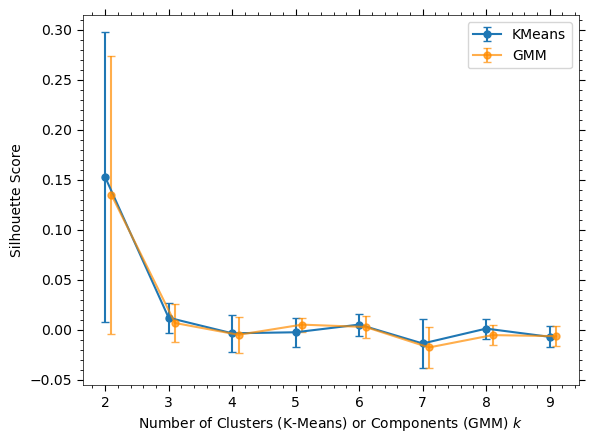
\includegraphics[width=0.9\textwidth]{./figures/q5a_silhouette_scores}
    \caption{The silhouette scores for the \inlinecode{KMeans} and \inlinecode{GaussianMixture} models on the pre-processed
        \inlinecode{ADS_baselineDataset.csv} dataset. 5 repetitions were performed to give a mean and standard deviation
        for each $k$ value.}
    \label{fig:q5a_silhouette_scores}
    \end{figure}

    \begin{figure}[htb]
    \centering
    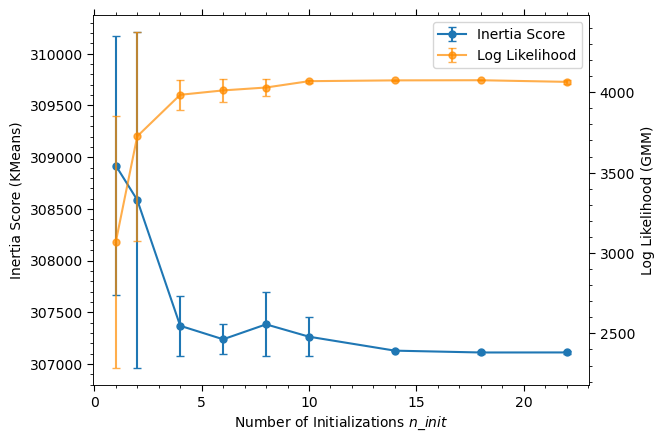
\includegraphics[width=0.9\textwidth]{./figures/q5a_n_init_optimisation}
    \caption{The cost functions for the \inlinecode{KMeans} and \inlinecode{GaussianMixture} models as \inlinecode{n_init} is
        increased, 5 repetitions were performed to give a mean and standard deviation for each \inlinecode{n_init} value.}
    \label{fig:q5a_n_init_optimisation}
    \end{figure}

    \begin{figure}[htb]
    \centering
    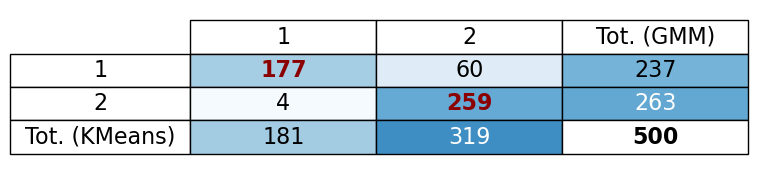
\includegraphics[width=0.9\textwidth]{./figures/q5a_contingency_table}
    \caption{A contingency table comparing cluster assignments for the \inlinecode{KMeans} and \inlinecode{GaussianMixture}
        models on the pre-processed \inlinecode{ADS_baselineDataset.csv} dataset, with $k=2$ and $n\_init=50$. The leading diagonal
        gives an 87.2\% agreement between the two models.}
    \label{fig:q5a_contingency_table}
    \end{figure}

    The dataset \inlinecode{ADS_baselineDataset.csv} underwent identical pre-processing as for Q4, followed by
    the application of K-Means and Gaussian Mixture Models.
    \inlinecode{KMeans}, employing Lloyd's algorithm, produces $k$ centroids, assigning each sample to the closest centroid,
    working under the assumption of a spherical data distribution.
    Conversely, \inlinecode{GaussianMixture} uses the expectation-maximisation algorithm to generate $k$ Gaussian
    distributions, assigning samples based on highest probability.
    This allows for greater flexibility due to the Gaussian distributions' ability to model spherical and non-spherical
    data.

    Fig. \eqref{fig:q5a_silhouette_scores} displays the silhouette scores for both models, suggesting $k=2$ as the optimal
    cluster number.
    However, significant errors at $k=2$ highlight instability in locating a consistent solution for both models,
    as such, Fig. \eqref{fig:q5a_n_init_optimisation} examines the impact of increased initialisations on the cost function for both models.
    Both algorithms are very dependent on the random initialisation of the centroids/distributions and the disappearance
    of the error bars on both models at $n\_init > 10$ indicated that the algorithms required at least this many random
    initialisations to find the global minima.
    Therefore, $n\_init=50$ was used hereon.

    Fig. \eqref{fig:q5a_contingency_table} presents a contingency table comparing cluster assignments of K-Means and
    Gaussian Mixture Models with these parameters, yielding an 87.2\% agreement.

\subsubsection{Question 5b}\label{subsubsec:q5b}
    \begin{figure}[htb]
    \centering
    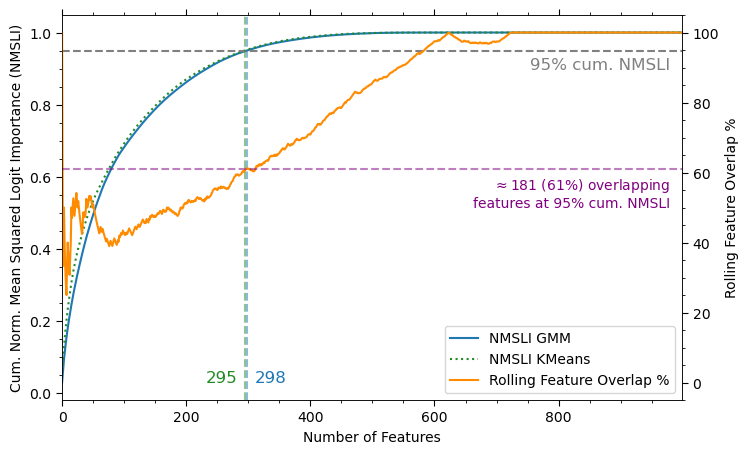
\includegraphics[width=0.9\textwidth]{./figures/q5b_feature_importance}
    \caption{The feature importance for the \inlinecode{KMeans} and \inlinecode{GaussianMixture} models using a \inlinecode{LogisticRegression}
        classifier and the NMSLI metric on the classified data shown in Fig. \eqref{fig:q5a_contingency_table}.
        The 95\% NMSLI threshold selected 295 and 298 important features for \inlinecode{KMeans} and \inlinecode{GaussianMixture} respectively, and the
        orange line indicates that roughly 181 of these features were shared between the two models.}
    \label{fig:q5b_feature_importance}
    \end{figure}

    \begin{figure}[htb]
    \centering
    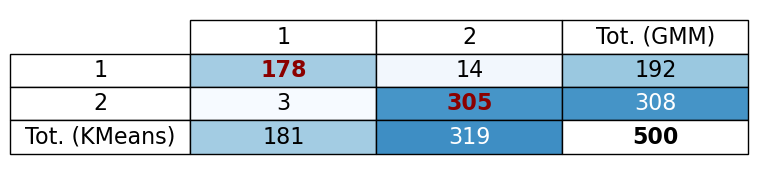
\includegraphics[width=0.9\textwidth]{./figures/q5b_contingency_table}
    \caption{A contingency table comparing cluster assignments for the \inlinecode{KMeans} and \inlinecode{GaussianMixture} models after feature
        reduction as shown in Fig. \eqref{fig:q5b_feature_importance}. The leading diagonal shows a 96.6\% agreement
        between the two models.}
    \label{fig:q5b_contingency_table}
    \end{figure}

    A \inlinecode{LogisticRegression} classifier was applied to the classifications in Fig. \eqref{fig:q5a_contingency_table} to
    assess feature importance using the NMSLI metric, detailed in Section \eqref{subsubsec:qf}.
    This is depicted in Fig. \eqref{fig:q5b_feature_importance}.
    Subsequently, the top 295 features for \inlinecode{KMeans} and 298 for \inlinecode{GaussianMixture} were employed to
    retrain both models.
    The resultant contingency table, shown in Fig. \eqref{fig:q5b_contingency_table}, indicates a significant improvement
    with 96.6\% agreement, surpassing the initial 87.2\% agreement observed in Fig. \eqref{fig:q5a_contingency_table}.

\subsubsection{Question 5c}\label{subsubsec:q5c}
    \begin{figure}[htb]
    \centering
    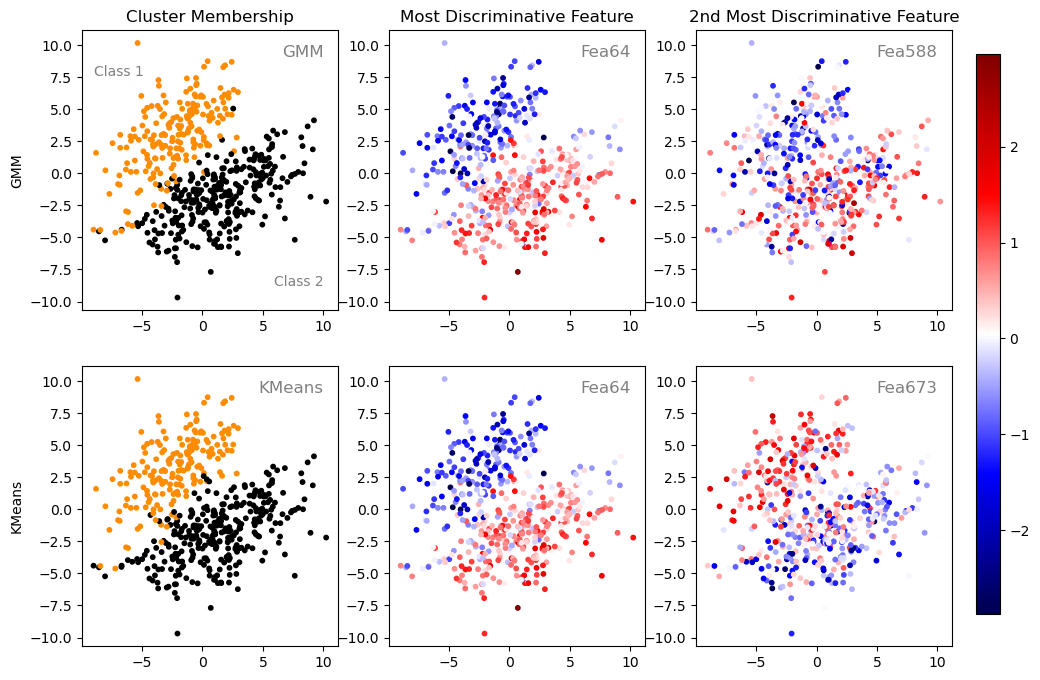
\includegraphics[width=0.9\textwidth]{./figures/q5c}
    \caption{PCA visualisations of the clusters found by the K-Means and Gaussian Mixture Models as shown in Fig.
        \eqref{fig:q5b_contingency_table}. The top row is for the \inlinecode{GaussianMixture} model and the bottom row is for the \inlinecode{KMeans} model.
        The left column shows the cluster membership, the middle and right columns show the samples coloured by the
        (standardised) first and second most discriminative features respectively. The x-axis is the first principal
        component and the y-axis is the second principal component for all plots.}
    \label{fig:q5c}
    \end{figure}

    Fig. \eqref{fig:q5c} presents the PCA visualisations of clusters identified by the k-means and Gaussian mixture models.
    The middle column reveals a strong positive correlation along $y=-x$ for the most discriminative feature, common to
    both models.
    In the right column, a slightly weaker positive correlation along the same line is shown for the second most
    discriminative feature in GMM, whereas this correlation is reversed for k-means.
    The second most discriminative feature differed between the two models.
